\documentclass[12pt]{beamer}

\beamertemplatenavigationsymbolsempty
\AtBeginSection[]
{
  \begin{frame}
    \frametitle{Table of Contents}
    \tableofcontents[currentsection]
  \end{frame}
}

\setlength{\tabcolsep}{10pt}

\title{Bipartite graphs}
\subtitle{Bipartite check, MCBM, MVC, MIS}
\author{beOI Training}
\institute{\includegraphics[height=12em]{../share/beoi-logo}}
\date{}
\usepackage[utf8]{inputenc}
\usepackage{listings}
\usepackage{tikz}
\usepackage{arrayjob}
\usepackage{amsmath}

% note: changed the color to make them "correct" on the beamer of La Marlagne
\definecolor{mygreen}{rgb}{0,1,0}
\definecolor{mygray}{rgb}{0.5,0.5,0.5}
\definecolor{mymauve}{rgb}{255,255,0}
\definecolor{myblue}{RGB}{0,0,255}
\definecolor{myred}{RGB}{255,255,0}
\definecolor{myblack}{RGB}{200,200,200}

\usetikzlibrary{decorations.pathmorphing,positioning,chains,fit,shapes,calc}
\tikzset{snake it/.style={decorate, decoration=snake}}
\tikzset{edgelabel/.style = {midway,rectangle, inner sep=0pt, draw=none, fill=white}}

\lstset{language=C++, basicstyle=\footnotesize}
\lstset{ %
  backgroundcolor=\color{white},   % choose the background color; you must add \usepackage{color} or \usepackage{xcolor}
  basicstyle=\tiny,  % the size of the fonts that are used for the code
  breakatwhitespace=false,   % sets if automatic breaks should only happen at whitespace
  breaklines=true,     % sets automatic line breaking
  commentstyle=\color{mygreen},    % comment style
  %deletekeywords={...},      % if you want to delete keywords from the given language
  escapeinside={\%*}{*)},    % if you want to add LaTeX within your code
  extendedchars=true,        % lets you use non-ASCII characters; for 8-bits encodings only, does not work with UTF-8
  frame=single,        % adds a frame around the code
  keepspaces=true,     % keeps spaces in text, useful for keeping indentation of code (possibly needs columns=flexible)
  keywordstyle=\color{blue},       % keyword style
  language=Java,     % the language of the code
  %morekeywords={*,...},      % if you want to add more keywords to the set
  numbers=left,        % where to put the line-numbers; possible values are (none, left, right)
  numbersep=5pt,       % how far the line-numbers are from the code
  numberstyle=\tiny\color{mygray}, % the style that is used for the line-numbers
  rulecolor=\color{black},   % if not set, the frame-color may be changed on line-breaks within not-black text (e.g. comments (green here))
  showspaces=false,    % show spaces everywhere adding particular underscores; it overrides 'showstringspaces'
  showstringspaces=false,    % underline spaces within strings only
  showtabs=false,      % show tabs within strings adding particular underscores
  stepnumber=1,        % the step between two line-numbers. If it's 1, each line will be numbered
  stringstyle=\color{mymauve},     % string literal style
  tabsize=2          % sets default tabsize to 2 spaces
}

\tikzstyle{vertex}=[circle,fill=gray!50,minimum size=15pt,inner sep=0pt]
\tikzstyle{visited}=[circle,fill=green!25,minimum size=15pt,inner sep=0pt]
\tikzstyle{unvisited}=[circle,fill=blue!25,minimum size=15pt,inner sep=0pt]


\tikzstyle{woman}=[circle,fill=pink!50,minimum size=15pt,inner sep=0pt]
\tikzstyle{men}=[circle,fill=blue!50,minimum size=15pt,inner sep=0pt]


\newcommand{\W}{\ {\color{red} \textbf{!!}} \ }

\begin{document}

\maketitle

\begin{frame}{Reminder about graphs}
  See 06-graph-basics
\end{frame}

\begin{frame}{Bipartite graphs}
  A graph is bipartite if it can be separated into two sets $U$ and $V$ such that nodes in $U$ are only connected to nodes in $V$, and conversely.
  
  \centering
  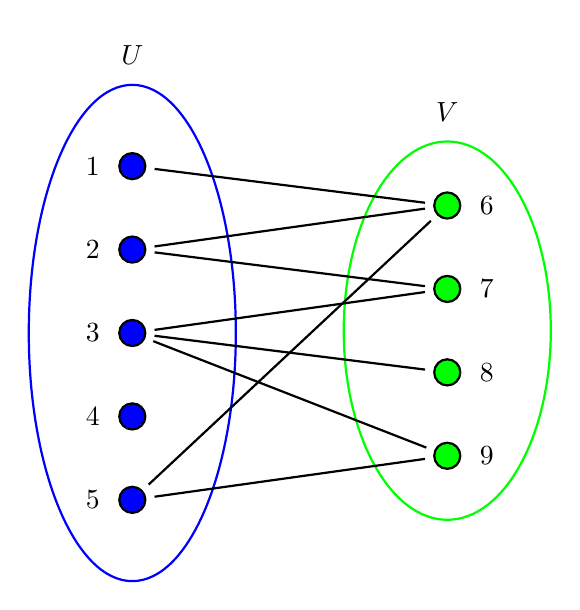
\begin{tikzpicture}[thick,
  every node/.style={draw,circle},
  fsnode/.style={fill=myblue},
  ssnode/.style={fill=mygreen},
  every fit/.style={ellipse,draw,inner sep=-2pt,text width=2cm},
  shorten >= 3pt,shorten <= 3pt
  ]
  
  % the vertices of U
  \begin{scope}[start chain=going below,node distance=7mm]
  \foreach \i in {1,2,...,5}
  \node[fsnode,on chain] (f\i) [label=left: \i] {};
  \end{scope}
  
  % the vertices of V
  \begin{scope}[xshift=4cm,yshift=-0.5cm,start chain=going below,node distance=7mm]
  \foreach \i in {6,7,...,9}
  \node[ssnode,on chain] (s\i) [label=right: \i] {};
  \end{scope}
  
  % the set U
  \node [myblue,fit=(f1) (f5),label=above:$U$] {};
  % the set V
  \node [mygreen,fit=(s6) (s9),label=above:$V$] {};
  
  % the edges
  \draw (f1) -- (s6);
  \draw (s6) -- (f2);
  \draw (f2) -- (s7);
  \draw (s7) -- (f3);
  \draw (s8) -- (f3);
  \draw (f3) -- (s9);
  \draw (s9) -- (f5);
  \draw (f5) -- (s6);
  \end{tikzpicture}
\end{frame}

\begin{frame}{A tree is also a bipartite graph}
  \begin{center}
    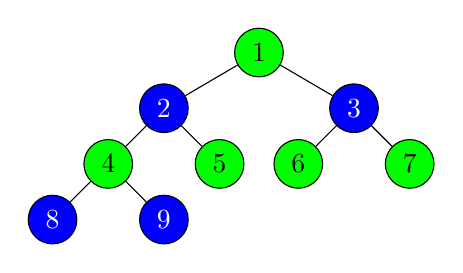
\begin{tikzpicture}[nodes={draw, circle}]
    \node (a8) [fill=mygreen] {1};
    \node (a6) [below left of = a8, xshift=-0.5cm, fill=myblue, text=white] {2};
    \node (a10) [below right of = a8, xshift=0.5cm, fill=myblue, text=white]{3};
    \node (a4) [below left of = a6, fill=mygreen]{4};
    \node (a7) [below right of = a6, fill=mygreen]{5};
    \node (a9) [below left of = a10, fill=mygreen]{6};
    \node (a11) [below right of = a10, fill=mygreen]{7};
    \node (a1) [below left of = a4, fill=myblue, text=white]{8};
    \node (n7) [below right of = a4, fill=myblue, text=white]{9};
    \draw (a8) -- (a10);
    \draw (a8) -- (a6); 
    \draw (a6) -- (a4);
    \draw (a6) -- (a7);
    \draw (a10) -- (a9);
    \draw (a10) -- (a11);
    \draw (a4) -- (a1);
    \draw (a4) -- (n7);
    \end{tikzpicture}
  \end{center}
  Here $U=\{1,4,5,6,7\}$ and $V=\{2,3,8,9\}$
\end{frame}

\begin{frame}{Weighted bipartite graphs}
  The same, but with weights:
  
  \centering
  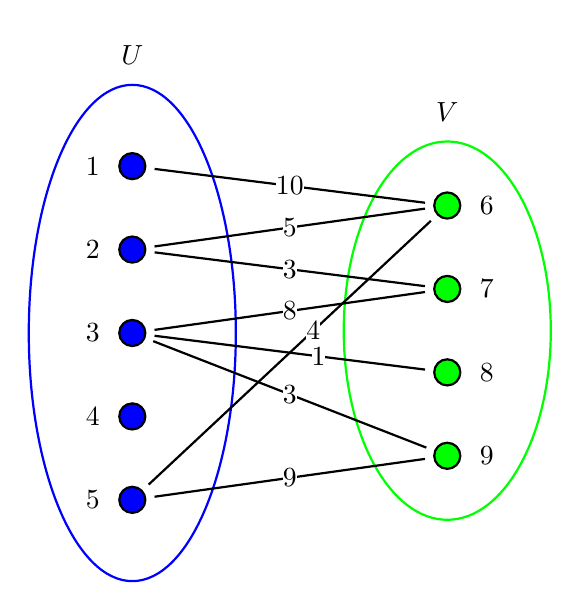
\begin{tikzpicture}[thick,
  every node/.style={draw,circle},
  fsnode/.style={fill=myblue},
  ssnode/.style={fill=mygreen},
  every fit/.style={ellipse,draw,inner sep=-2pt,text width=2cm},
  shorten >= 3pt,shorten <= 3pt
  ]
  
  % the vertices of U
  \begin{scope}[start chain=going below,node distance=7mm]
  \foreach \i in {1,2,...,5}
  \node[fsnode,on chain] (f\i) [label=left: \i] {};
  \end{scope}
  
  % the vertices of V
  \begin{scope}[xshift=4cm,yshift=-0.5cm,start chain=going below,node distance=7mm]
  \foreach \i in {6,7,...,9}
  \node[ssnode,on chain] (s\i) [label=right: \i] {};
  \end{scope}
  
  % the set U
  \node [myblue,fit=(f1) (f5),label=above:$U$] {};
  % the set V
  \node [mygreen,fit=(s6) (s9),label=above:$V$] {};
  
  % the edges
  \draw (f1) -- (s6) node [edgelabel] () {10};
  \draw (s6) -- (f2) node [edgelabel] () {5};
  \draw (f2) -- (s7) node [edgelabel] () {3};
  \draw (s7) -- (f3) node [edgelabel] () {8};
  \draw (s8) -- (f3) node [edgelabel,pos=0.4] () {1};
  \draw (f3) -- (s9) node [edgelabel] () {3};
  \draw (s9) -- (f5) node [edgelabel] () {9};
  \draw (f5) -- (s6) node [edgelabel,pos=0.58] () {4};
  \end{tikzpicture}
\end{frame}

\begin{frame}{Bipartite check}
  \begin{center}
    How to test if a particular graph is a bipartite one?
    \vspace{0.5cm}
    
    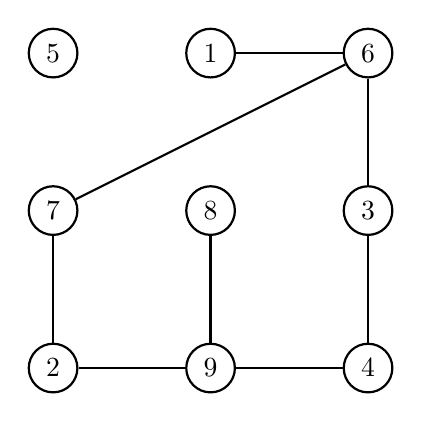
\begin{tikzpicture}[thick,
    every node/.style={draw,circle},
    fsnode/.style={fill=myblue},
    ssnode/.style={fill=mygreen},
    every fit/.style={ellipse,draw,inner sep=-2pt,text width=2cm},
    node distance=2cm
    ]
    
    \node (f1) [fill=white] {1};
    \node (f4) [fill=white,left of=f1] {5};
    \node (s6) [fill=white,right of=f1] {6};
    \node (f5) [fill=white,below of=f4] {7};
    \node (s8) [fill=white,below of=f1] {8};
    \node (f2) [fill=white,below of=s6] {3};
    \node (f3) [fill=white,below of=s8] {9};
    \node (s7) [fill=white,below of=f2] {4};
    \node (s9) [fill=white,below of=f5] {2};
    
    % the edges
    \draw (f1) -- (s6);
    \draw (s6) -- (f2);
    \draw (f2) -- (s7);
    \draw (s7) -- (f3);
    \draw (s8) -- (f3);
    \draw (f3) -- (s9);
    \draw (s9) -- (f5);
    \draw (f5) -- (s6);
    \end{tikzpicture}
    \vspace{0.5cm}
    
    \pause DFS with coloration!
  \end{center}
\end{frame}

\begin{frame}{Bipartite check}
  \begin{center}
    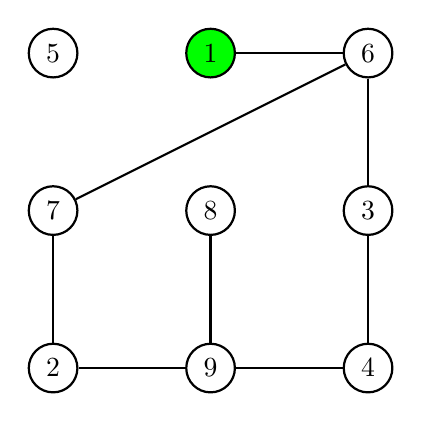
\begin{tikzpicture}[thick,
    every node/.style={draw,circle},
    fsnode/.style={fill=myblue},
    ssnode/.style={fill=mygreen},
    every fit/.style={ellipse,draw,inner sep=-2pt,text width=2cm},
    node distance=2cm
    ]
    
    \node (f1) [fill=mygreen] {1};
    \node (f4) [fill=white,left of=f1] {5};
    \node (s6) [fill=white,right of=f1] {6};
    \node (f5) [fill=white,below of=f4] {7};
    \node (s8) [fill=white,below of=f1] {8};
    \node (f2) [fill=white,below of=s6] {3};
    \node (f3) [fill=white,below of=s8] {9};
    \node (s7) [fill=white,below of=f2] {4};
    \node (s9) [fill=white,below of=f5] {2};
    
    % the edges
    \draw (f1) -- (s6);
    \draw (s6) -- (f2);
    \draw (f2) -- (s7);
    \draw (s7) -- (f3);
    \draw (s8) -- (f3);
    \draw (f3) -- (s9);
    \draw (s9) -- (f5);
    \draw (f5) -- (s6);
    \end{tikzpicture}
  \end{center}
\end{frame}

\begin{frame}{Bipartite check}
  \begin{center}
    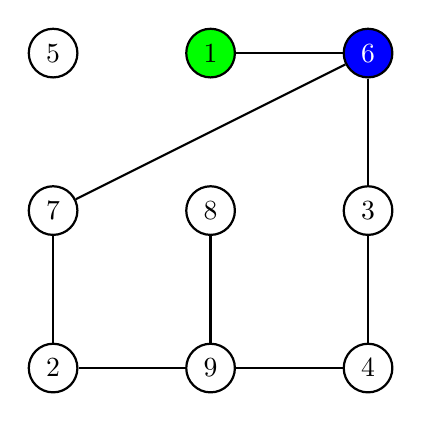
\begin{tikzpicture}[thick,
    every node/.style={draw,circle},
    fsnode/.style={fill=myblue},
    ssnode/.style={fill=mygreen},
    every fit/.style={ellipse,draw,inner sep=-2pt,text width=2cm},
    node distance=2cm
    ]
    
    \node (f1) [fill=mygreen] {1};
    \node (f4) [fill=white,left of=f1] {5};
    \node (s6) [fill=myblue,right of=f1,text=white] {6};
    \node (f5) [fill=white,below of=f4] {7};
    \node (s8) [fill=white,below of=f1] {8};
    \node (f2) [fill=white,below of=s6] {3};
    \node (f3) [fill=white,below of=s8] {9};
    \node (s7) [fill=white,below of=f2] {4};
    \node (s9) [fill=white,below of=f5] {2};
    
    % the edges
    \draw (f1) -- (s6);
    \draw (s6) -- (f2);
    \draw (f2) -- (s7);
    \draw (s7) -- (f3);
    \draw (s8) -- (f3);
    \draw (f3) -- (s9);
    \draw (s9) -- (f5);
    \draw (f5) -- (s6);
    \end{tikzpicture}
  \end{center}
\end{frame}

\begin{frame}{Bipartite check}
  \begin{center}
    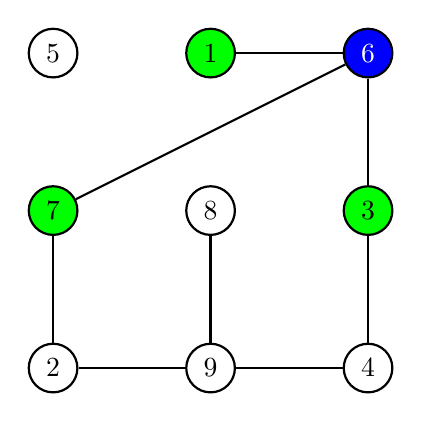
\begin{tikzpicture}[thick,
    every node/.style={draw,circle},
    fsnode/.style={fill=myblue},
    ssnode/.style={fill=mygreen},
    every fit/.style={ellipse,draw,inner sep=-2pt,text width=2cm},
    node distance=2cm
    ]
    
    \node (f1) [fill=mygreen] {1};
    \node (f4) [fill=white,left of=f1] {5};
    \node (s6) [fill=myblue,right of=f1,text=white] {6};
    \node (f5) [fill=mygreen,below of=f4] {7};
    \node (s8) [fill=white,below of=f1] {8};
    \node (f2) [fill=mygreen,below of=s6] {3};
    \node (f3) [fill=white,below of=s8] {9};
    \node (s7) [fill=white,below of=f2] {4};
    \node (s9) [fill=white,below of=f5] {2};
    
    % the edges
    \draw (f1) -- (s6);
    \draw (s6) -- (f2);
    \draw (f2) -- (s7);
    \draw (s7) -- (f3);
    \draw (s8) -- (f3);
    \draw (f3) -- (s9);
    \draw (s9) -- (f5);
    \draw (f5) -- (s6);
    \end{tikzpicture}
  \end{center}
\end{frame}

\begin{frame}{Bipartite check}
  \begin{center}
    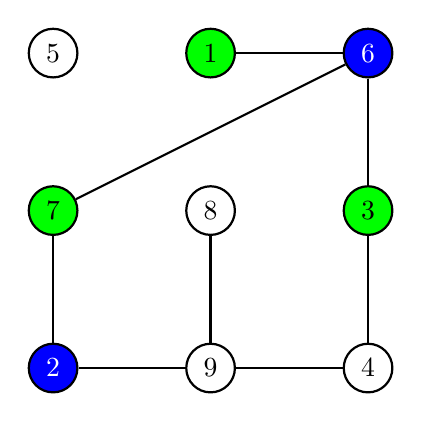
\begin{tikzpicture}[thick,
    every node/.style={draw,circle},
    fsnode/.style={fill=myblue},
    ssnode/.style={fill=mygreen},
    every fit/.style={ellipse,draw,inner sep=-2pt,text width=2cm},
    node distance=2cm
    ]
    
    \node (f1) [fill=mygreen] {1};
    \node (f4) [fill=white,left of=f1] {5};
    \node (s6) [fill=myblue,right of=f1,text=white] {6};
    \node (f5) [fill=mygreen,below of=f4] {7};
    \node (s8) [fill=white,below of=f1] {8};
    \node (f2) [fill=mygreen,below of=s6] {3};
    \node (f3) [fill=white,below of=s8] {9};
    \node (s7) [fill=white,below of=f2] {4};
    \node (s9) [fill=myblue,below of=f5,text=white] {2};
    
    % the edges
    \draw (f1) -- (s6);
    \draw (s6) -- (f2);
    \draw (f2) -- (s7);
    \draw (s7) -- (f3);
    \draw (s8) -- (f3);
    \draw (f3) -- (s9);
    \draw (s9) -- (f5);
    \draw (f5) -- (s6);
    \end{tikzpicture}
  \end{center}
\end{frame}

\begin{frame}{Bipartite check}
  \begin{center}
    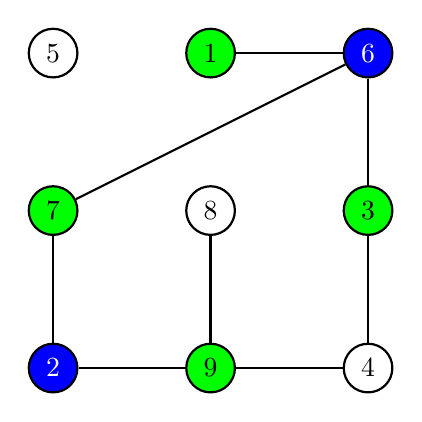
\begin{tikzpicture}[thick,
    every node/.style={draw,circle},
    fsnode/.style={fill=myblue},
    ssnode/.style={fill=mygreen},
    every fit/.style={ellipse,draw,inner sep=-2pt,text width=2cm},
    node distance=2cm
    ]
    
    \node (f1) [fill=mygreen] {1};
    \node (f4) [fill=white,left of=f1] {5};
    \node (s6) [fill=myblue,right of=f1,text=white] {6};
    \node (f5) [fill=mygreen,below of=f4] {7};
    \node (s8) [fill=white,below of=f1] {8};
    \node (f2) [fill=mygreen,below of=s6] {3};
    \node (f3) [fill=mygreen,below of=s8] {9};
    \node (s7) [fill=white,below of=f2] {4};
    \node (s9) [fill=myblue,below of=f5,text=white] {2};
    
    % the edges
    \draw (f1) -- (s6);
    \draw (s6) -- (f2);
    \draw (f2) -- (s7);
    \draw (s7) -- (f3);
    \draw (s8) -- (f3);
    \draw (f3) -- (s9);
    \draw (s9) -- (f5);
    \draw (f5) -- (s6);
    \end{tikzpicture}
  \end{center}
\end{frame}

\begin{frame}{Bipartite check}
  \begin{center}
    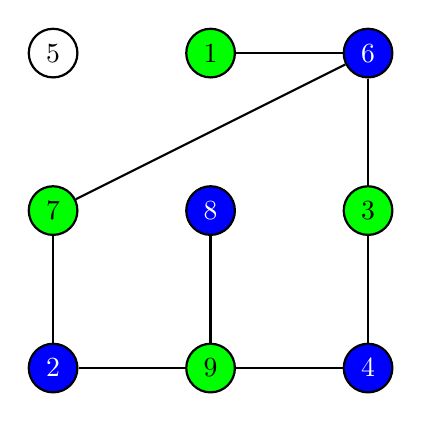
\begin{tikzpicture}[thick,
    every node/.style={draw,circle},
    fsnode/.style={fill=myblue},
    ssnode/.style={fill=mygreen},
    every fit/.style={ellipse,draw,inner sep=-2pt,text width=2cm},
    node distance=2cm
    ]
    
    \node (f1) [fill=mygreen] {1};
    \node (f4) [fill=white,left of=f1] {5};
    \node (s6) [fill=myblue,right of=f1,text=white] {6};
    \node (f5) [fill=mygreen,below of=f4] {7};
    \node (s8) [fill=myblue,below of=f1,text=white] {8};
    \node (f2) [fill=mygreen,below of=s6] {3};
    \node (f3) [fill=mygreen,below of=s8] {9};
    \node (s7) [fill=myblue,below of=f2,text=white] {4};
    \node (s9) [fill=myblue,below of=f5,text=white] {2};
    
    % the edges
    \draw (f1) -- (s6);
    \draw (s6) -- (f2);
    \draw (f2) -- (s7);
    \draw (s7) -- (f3);
    \draw (s8) -- (f3);
    \draw (f3) -- (s9);
    \draw (s9) -- (f5);
    \draw (f5) -- (s6);
    \end{tikzpicture}
  \end{center}
\end{frame}

\begin{frame}{Bipartite check}
  \begin{center}
    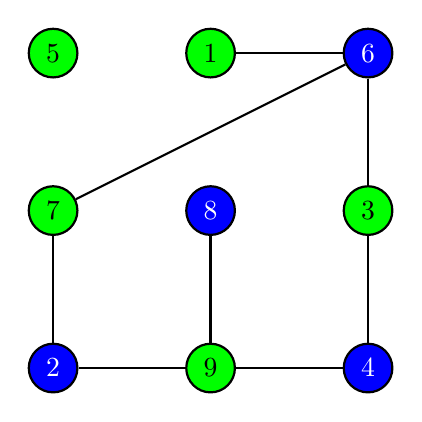
\begin{tikzpicture}[thick,
    every node/.style={draw,circle},
    fsnode/.style={fill=myblue},
    ssnode/.style={fill=mygreen},
    every fit/.style={ellipse,draw,inner sep=-2pt,text width=2cm},
    node distance=2cm
    ]
    
    \node (f1) [fill=mygreen] {1};
    \node (f4) [fill=mygreen,left of=f1] {5};
    \node (s6) [fill=myblue,right of=f1,text=white] {6};
    \node (f5) [fill=mygreen,below of=f4] {7};
    \node (s8) [fill=myblue,below of=f1,text=white] {8};
    \node (f2) [fill=mygreen,below of=s6] {3};
    \node (f3) [fill=mygreen,below of=s8] {9};
    \node (s7) [fill=myblue,below of=f2,text=white] {4};
    \node (s9) [fill=myblue,below of=f5,text=white] {2};
    
    % the edges
    \draw (f1) -- (s6);
    \draw (s6) -- (f2);
    \draw (f2) -- (s7);
    \draw (s7) -- (f3);
    \draw (s8) -- (f3);
    \draw (f3) -- (s9);
    \draw (s9) -- (f5);
    \draw (f5) -- (s6);
    \end{tikzpicture}
  \end{center}
  Ok!
\end{frame}

\begin{frame}[fragile]{Algorithm}
  \begin{lstlisting}
bool visit(int, const vector<vector<int>>&, vector<int>&, int); // defined below

bool isBipartite(int n, const vector<vector<int>>& successors) {
    //successors[i] contains the successors of node i
    vector<int> color(n, -1); // initialized to -1

    for (int i = 0; i < n; i++) {
        if (color[i] == -1)
            if (!visit(i, successors, color, 1))
                return false;
    }
    return true;
}

bool visit(int node, const vector<vector<int>>& successors, vector<int>& color, int parentColor) {
    if (color[node] == parentColor) // failure
        return false;

    if (color[node] != -1) // avoid infinite looping
        return true;

    color[node] = (parentColor + 1) % 2;
    for (int next : successors[node])
        if (!visit(next, successors, node, color[node]))
            return false;
    return true;
}
  \end{lstlisting}
\end{frame}

\begin{frame}{Maximum Cardinality Bipartite Matching}
    Given a set $U$ of men and a set $V$ of women, and a list of "compatibilities" between men and women, we obtain this:
    \centering
    \scalebox{0.8}{
    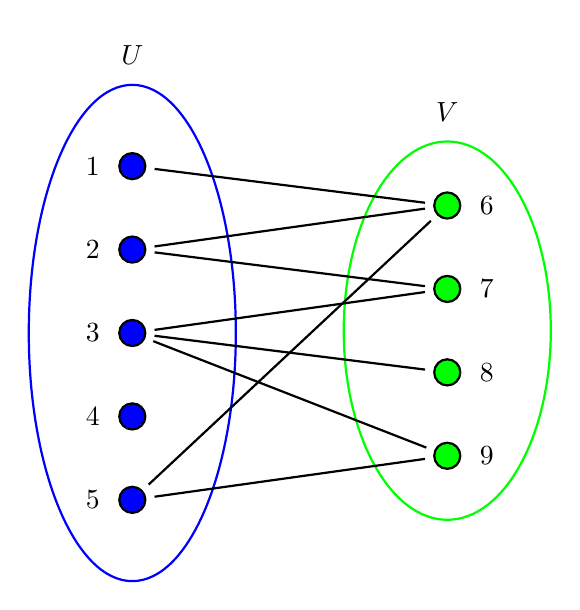
\begin{tikzpicture}[thick,
    every node/.style={draw,circle},
    fsnode/.style={fill=myblue},
    ssnode/.style={fill=mygreen},
    every fit/.style={ellipse,draw,inner sep=-2pt,text width=2cm},
    shorten >= 3pt,shorten <= 3pt
    ]
    
    % the vertices of U
    \begin{scope}[start chain=going below,node distance=7mm]
    \foreach \i in {1,2,...,5}
    \node[fsnode,on chain] (f\i) [label=left: \i] {};
    \end{scope}
    
    % the vertices of V
    \begin{scope}[xshift=4cm,yshift=-0.5cm,start chain=going below,node distance=7mm]
    \foreach \i in {6,7,...,9}
    \node[ssnode,on chain] (s\i) [label=right: \i] {};
    \end{scope}
    
    % the set U
    \node [myblue,fit=(f1) (f5),label=above:$U$] {};
    % the set V
    \node [mygreen,fit=(s6) (s9),label=above:$V$] {};
    
    % the edges
    \draw (f1) -- (s6);
    \draw (s6) -- (f2);
    \draw (f2) -- (s7);
    \draw (s7) -- (f3);
    \draw (s8) -- (f3);
    \draw (f3) -- (s9);
    \draw (s9) -- (f5);
    \draw (f5) -- (s6);
    \end{tikzpicture}}
    
    Can you create a maximum number of couples?
\end{frame}

\begin{frame}{A bit of theory}
    $M\in E$ is a \textbf{matching} if each node is used at most once by the edges in $M$.
    \vspace{1cm}
    
    A \textbf{maximum cardinality matching} is a matching that has the maximal number of edge/node possible.
    \vspace{1cm}
    
    A node which is not used by any edge in a matching is said \textbf{free}. The others are said \textbf{non-free}.
\end{frame}

\begin{frame}{An example of matching}
    \centering
    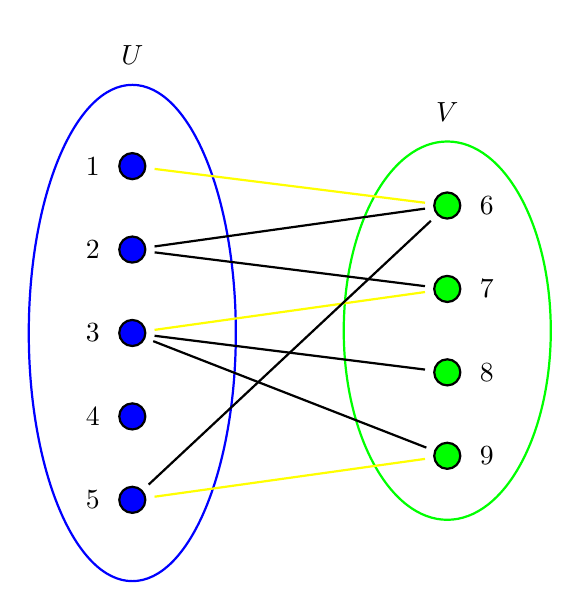
\begin{tikzpicture}[thick,
    every node/.style={draw,circle},
    fsnode/.style={fill=myblue},
    ssnode/.style={fill=mygreen},
    every fit/.style={ellipse,draw,inner sep=-2pt,text width=2cm},
    shorten >= 3pt,shorten <= 3pt
    ]
    
    % the vertices of U
    \begin{scope}[start chain=going below,node distance=7mm]
    \foreach \i in {1,2,...,5}
    \node[fsnode,on chain] (f\i) [label=left: \i] {};
    \end{scope}
    
    % the vertices of V
    \begin{scope}[xshift=4cm,yshift=-0.5cm,start chain=going below,node distance=7mm]
    \foreach \i in {6,7,...,9}
    \node[ssnode,on chain] (s\i) [label=right: \i] {};
    \end{scope}
    
    % the set U
    \node [myblue,fit=(f1) (f5),label=above:$U$] {};
    % the set V
    \node [mygreen,fit=(s6) (s9),label=above:$V$] {};
    
    % the edges
    \draw (f1) -- (s6) [color=myred];
    \draw (s6) -- (f2);
    \draw (f2) -- (s7);
    \draw (s7) -- (f3) [color=myred];
    \draw (s8) -- (f3);
    \draw (f3) -- (s9);
    \draw (s9) -- (f5) [color=myred];
    \draw (f5) -- (s6);
    \end{tikzpicture}
    
    It is maximal?
    \pause How to improve it?
\end{frame}

\begin{frame}{More theory}
    An augmenting path for a matching $M$ is a path starting and ending at free nodes, and alternating between matched and unmatched edges.
\end{frame}

\begin{frame}{An example of augmenting path}
    \centering
    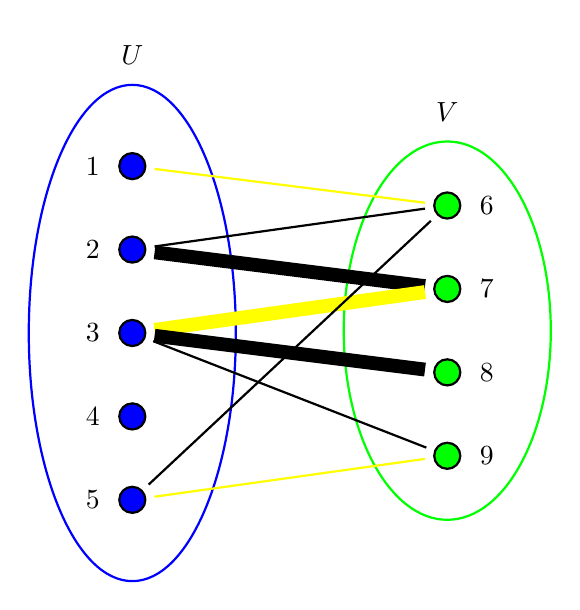
\begin{tikzpicture}[thick,
    every node/.style={draw,circle},
    fsnode/.style={fill=myblue},
    ssnode/.style={fill=mygreen},
    every fit/.style={ellipse,draw,inner sep=-2pt,text width=2cm},
    shorten >= 3pt,shorten <= 3pt
    ]
    
    % the vertices of U
    \begin{scope}[start chain=going below,node distance=7mm]
    \foreach \i in {1,2,...,5}
    \node[fsnode,on chain] (f\i) [label=left: \i] {};
    \end{scope}
    
    % the vertices of V
    \begin{scope}[xshift=4cm,yshift=-0.5cm,start chain=going below,node distance=7mm]
    \foreach \i in {6,7,...,9}
    \node[ssnode,on chain] (s\i) [label=right: \i] {};
    \end{scope}
    
    % the set U
    \node [myblue,fit=(f1) (f5),label=above:$U$] {};
    % the set V
    \node [mygreen,fit=(s6) (s9),label=above:$V$] {};
    
    % the edges
    \draw (f1) -- (s6) [color=myred];
    \draw (s6) -- (f2) ;
    \draw (f2) -- (s7) [line width=5pt];
    \draw (s7) -- (f3) [color=myred,line width=5pt];
    \draw (s8) -- (f3) [line width=5pt];
    \draw (f3) -- (s9) ;
    \draw (s9) -- (f5) [color=myred];
    \draw (f5) -- (s6);
    \end{tikzpicture}
\end{frame}

\begin{frame}{Let's think about augmenting paths}
    \centering
    \scalebox{0.35}{
        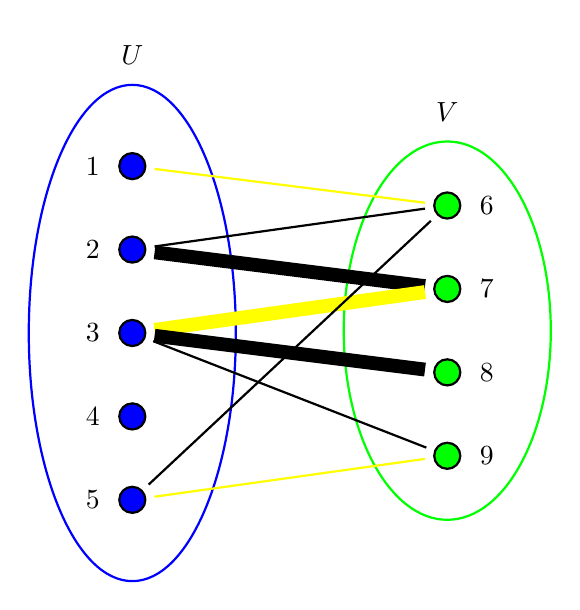
\begin{tikzpicture}[thick,
        every node/.style={draw,circle},
        fsnode/.style={fill=myblue},
        ssnode/.style={fill=mygreen},
        every fit/.style={ellipse,draw,inner sep=-2pt,text width=2cm},
        shorten >= 3pt,shorten <= 3pt
        ]
        
        % the vertices of U
        \begin{scope}[start chain=going below,node distance=7mm]
        \foreach \i in {1,2,...,5}
        \node[fsnode,on chain] (f\i) [label=left: \i] {};
        \end{scope}
        
        % the vertices of V
        \begin{scope}[xshift=4cm,yshift=-0.5cm,start chain=going below,node distance=7mm]
        \foreach \i in {6,7,...,9}
        \node[ssnode,on chain] (s\i) [label=right: \i] {};
        \end{scope}
        
        % the set U
        \node [myblue,fit=(f1) (f5),label=above:$U$] {};
        % the set V
        \node [mygreen,fit=(s6) (s9),label=above:$V$] {};
        
        % the edges
        \draw (f1) -- (s6) [color=myred];
        \draw (s6) -- (f2) ;
        \draw (f2) -- (s7) [line width=5pt];
        \draw (s7) -- (f3) [color=myred,line width=5pt];
        \draw (s8) -- (f3) [line width=5pt];
        \draw (f3) -- (s9) ;
        \draw (s9) -- (f5) [color=myred];
        \draw (f5) -- (s6);
        \end{tikzpicture}
    }
    
    How can we use such paths? Let's find some useful properties
    \begin{itemize}
        \pause \item By definition, an aug. path always starts and ends at a free node
        \pause \item Thus, the first and last edge are not in $M$
        \pause \item The size of an aug. path is always odd
        \pause \item There is always one "free edge" more than the number of "taken edges" in an aug. path
        \pause \item What if we inverse the edges?
    \end{itemize}
\end{frame}

\begin{frame}{An augmenting path}
    \centering
    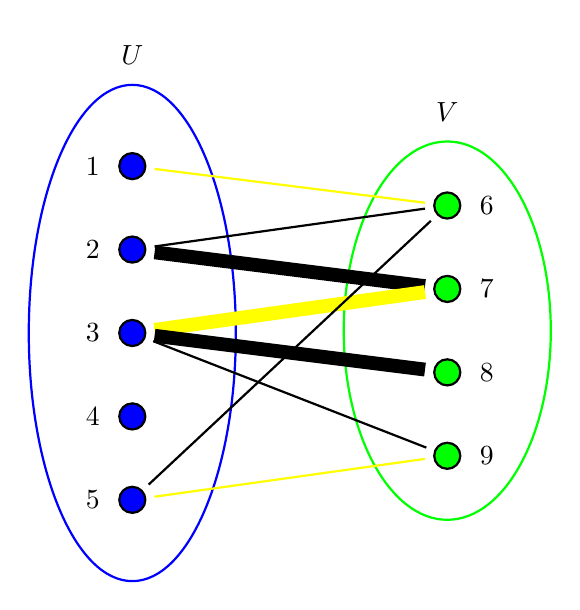
\begin{tikzpicture}[thick,
    every node/.style={draw,circle},
    fsnode/.style={fill=myblue},
    ssnode/.style={fill=mygreen},
    every fit/.style={ellipse,draw,inner sep=-2pt,text width=2cm},
    shorten >= 3pt,shorten <= 3pt
    ]
    
    % the vertices of U
    \begin{scope}[start chain=going below,node distance=7mm]
    \foreach \i in {1,2,...,5}
    \node[fsnode,on chain] (f\i) [label=left: \i] {};
    \end{scope}
    
    % the vertices of V
    \begin{scope}[xshift=4cm,yshift=-0.5cm,start chain=going below,node distance=7mm]
    \foreach \i in {6,7,...,9}
    \node[ssnode,on chain] (s\i) [label=right: \i] {};
    \end{scope}
    
    % the set U
    \node [myblue,fit=(f1) (f5),label=above:$U$] {};
    % the set V
    \node [mygreen,fit=(s6) (s9),label=above:$V$] {};
    
    % the edges
    \draw (f1) -- (s6) [color=myred];
    \draw (s6) -- (f2) ;
    \draw (f2) -- (s7) [line width=5pt];
    \draw (s7) -- (f3) [color=myred,line width=5pt];
    \draw (s8) -- (f3) [line width=5pt];
    \draw (f3) -- (s9) ;
    \draw (s9) -- (f5) [color=myred];
    \draw (f5) -- (s6);
    \end{tikzpicture}
\end{frame}

\begin{frame}{Inversing the augmenting path}
    \centering
    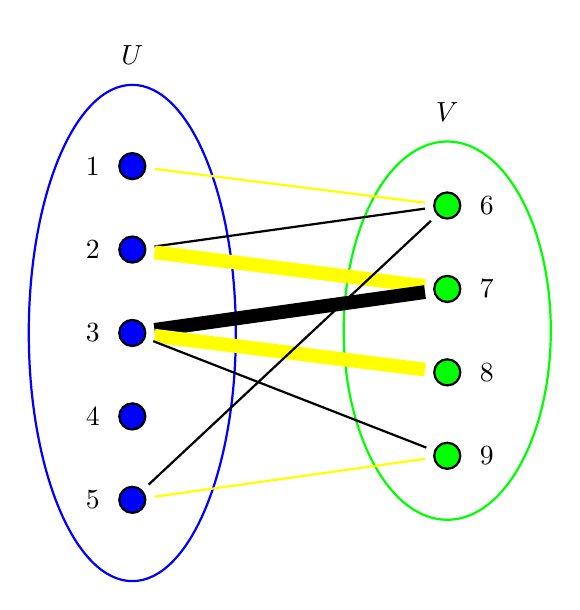
\begin{tikzpicture}[thick,
    every node/.style={draw,circle},
    fsnode/.style={fill=myblue},
    ssnode/.style={fill=mygreen},
    every fit/.style={ellipse,draw,inner sep=-2pt,text width=2cm},
    shorten >= 3pt,shorten <= 3pt
    ]
    
    % the vertices of U
    \begin{scope}[start chain=going below,node distance=7mm]
    \foreach \i in {1,2,...,5}
    \node[fsnode,on chain] (f\i) [label=left: \i] {};
    \end{scope}
    
    % the vertices of V
    \begin{scope}[xshift=4cm,yshift=-0.5cm,start chain=going below,node distance=7mm]
    \foreach \i in {6,7,...,9}
    \node[ssnode,on chain] (s\i) [label=right: \i] {};
    \end{scope}
    
    % the set U
    \node [myblue,fit=(f1) (f5),label=above:$U$] {};
    % the set V
    \node [mygreen,fit=(s6) (s9),label=above:$V$] {};
    
    % the edges
    \draw (f1) -- (s6) [color=myred];
    \draw (s6) -- (f2) ;
    \draw (f2) -- (s7) [color=myred,line width=5pt];
    \draw (s7) -- (f3) [line width=5pt];
    \draw (s8) -- (f3) [color=myred,line width=5pt];
    \draw (f3) -- (s9) ;
    \draw (s9) -- (f5) [color=myred];
    \draw (f5) -- (s6);
    \end{tikzpicture}
\end{frame}

\begin{frame}{Augmenting path = good?}
    \begin{itemize}
        \item It is always possible to inverse an augmenting path
        \item It always increase the size of the matching by 1!
    \end{itemize}
\end{frame}

\begin{frame}{Augmenting path = good!}
    Given a matching $M$ in a bipartite graph such that there exist no augmenting path, then $M$ is of \textbf{maximal cardinality}.
\end{frame}

\begin{frame}{Solving the MCBM}
    \begin{enumerate}
        \item Find an aug. path. If no such path exists, return the matching, it is maximal
        \item Inverse the path found
        \item Repeat from 1
    \end{enumerate}
    
    Simple, isn't it?
\end{frame}

\begin{frame}{Let's see two algorithms}
    \begin{itemize}
        \item The first one is based on the "flow" representation of the graph, and is very similar to a max flow. Simple to understand, but longer.
        \item The second is recursive so more difficult to understand but shorter.
    \end{itemize}
\end{frame}

\begin{frame}{Finding an aug. path}
    An alternative representation:
    \centering
    \scalebox{0.9}{
    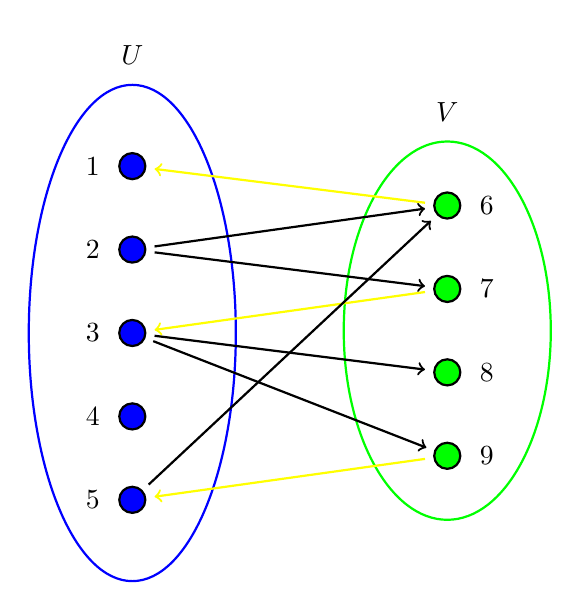
\begin{tikzpicture}[thick,
    every node/.style={draw,circle},
    fsnode/.style={fill=myblue},
    ssnode/.style={fill=mygreen},
    every fit/.style={ellipse,draw,inner sep=-2pt,text width=2cm},
    shorten >= 3pt,shorten <= 3pt
    ]
    
    % the vertices of U
    \begin{scope}[start chain=going below,node distance=7mm]
    \foreach \i in {1,2,...,5}
    \node[fsnode,on chain] (f\i) [label=left: \i] {};
    \end{scope}
    
    % the vertices of V
    \begin{scope}[xshift=4cm,yshift=-0.5cm,start chain=going below,node distance=7mm]
    \foreach \i in {6,7,...,9}
    \node[ssnode,on chain] (s\i) [label=right: \i] {};
    \end{scope}
    
    % the set U
    \node [myblue,fit=(f1) (f5),label=above:$U$] {};
    % the set V
    \node [mygreen,fit=(s6) (s9),label=above:$V$] {};
    
    % the edges
    \draw (f1) -- (s6) [<-,color=myred];
    \draw (s6) -- (f2) [<-];
    \draw (f2) -- (s7) [->];
    \draw (s7) -- (f3) [->,color=myred];
    \draw (s8) -- (f3) [<-];
    \draw (f3) -- (s9) [->];
    \draw (s9) -- (f5) [->,color=myred];
    \draw (f5) -- (s6) [->];
    \end{tikzpicture}}

    In this representation, an aug. path is a path starting at a free node in $U$ and ending at a free node in $V$.
\end{frame}

\begin{frame}[fragile]{Finding an aug. path}
    \begin{lstlisting}
// succ[i] contains the nodes that can be reached from i
// initially, all the edges are from U->V
// inU[i] is true iff i is in U 
bool findAndReverse(int n, vector<vector<int>>& succ, vector<bool>& inU) {
    vector<int> pred(n);
    vector<bool> visited(n, false);
    stack<int> todo;
    
    // Find free nodes in U
    vector<bool> isFree(n, true);
    for (int i = 0; i < n; i++)
        if (!inU[i])
            for (int s : succ[i])
                    isFree[s] = false;

    for (int i = 0; i < n; i++) {
        if (inU[i] && isFree[i]) {
            todo.push(i);
            pred[i] = -1;
        }
    }\end{lstlisting}
\end{frame}

\begin{frame}[fragile]{Finding an aug. path (cont.)}
    \begin{lstlisting}[firstnumber=23]
    // Run the DFS
    int found = -1;
    while(!todo.empty()) {
        int node = todo.top(); todo.pop();
        if(visited[node])
            continue;
        visited[node] = true;
        //if we are at a free node in V
        if(!inU[node] && succ[node].size() == 0) {
            found = node;
            break;
        }
        else {
            for(int next: successors[node]) {
                if(!visited[next]) {
                    pred[next] = node;
                    todo.push(next);
                }
            }
        }
    }
    
    // Reverse the nodes
    if(found != -1) {
        while(predecessors[found] != -1) {
            succ[pred[found]].erase(found);
            succ[found].push_back(pred[found]);
            found = pred[found];
        }
        return true;
    }
    return false;
}\end{lstlisting}
\end{frame}

\begin{frame}[fragile]{Final algorithm}
\begin{lstlisting}
void getMCBM(int n, vector<vector<int>>& succ, vector<bool>& inU) {
    while(findAndReverse(n, succ, inU)) {}
    //MCBM == edges from nodes in V (in succ)
}\end{lstlisting}
\end{frame}

\begin{frame}[fragile]{Another (shorter) algorithm}
    \begin{lstlisting}[language=C++]
vector<vi> AdjList;
vi match, vis;

int Aug(int l) { // return 1 if an augmenting path is found
    if (vis[l]) return 0; // return 0 otherwise
    vis[l] = 1;
    for (int j = 0; j < (int)AdjList[l].size(); j++) {
        int r = AdjList[l][j];
        if (match[r] == -1 || Aug(match[r])) {
            match[r] = l; 
            return 1; // found 1 matching
        }
    }
    return 0; // no matching
}

int MCBM = 0;
match.assign(V, -1); //V = total number of vertices
for(int l = 0; l < n; l++) { //n = size of the left set
    vis.assign(n, 0);
    MCBM += Aug(l);
}\end{lstlisting}
\end{frame}

\begin{frame}{Minimum vertex cover (in bipartite graph)}
    A \textbf{Vertex cover} $K$ is a set of nodes from $G$ such that each edge of $G$ is incident to at least one node of $K$.
    
    A \textbf{Minimal vertex cover} is a vertex cover of minimal size.\\
    
    \centering
    \scalebox{0.8}{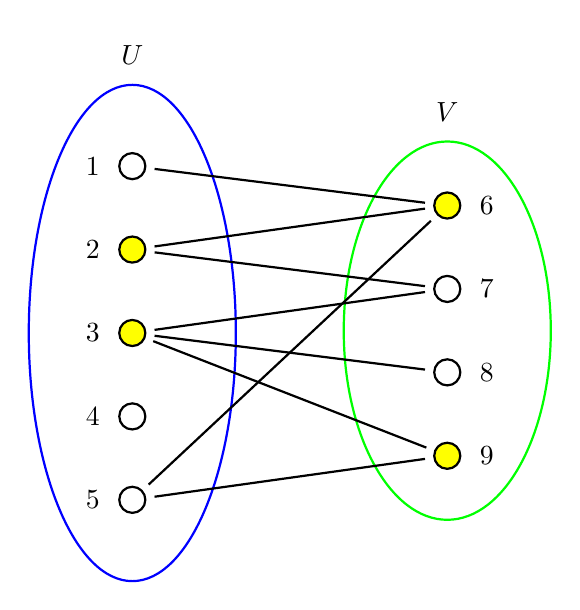
\begin{tikzpicture}[thick,
    every node/.style={draw,circle},
    fsnode/.style={fill=myblue},
    ssnode/.style={fill=mygreen},
    every fit/.style={ellipse,draw,inner sep=-2pt,text width=2cm},
    shorten >= 3pt,shorten <= 3pt
    ]
    
    % the vertices of U
    \begin{scope}[start chain=going below,node distance=7mm]
    \node[fsnode,on chain,fill=white] (f1) [label=left: 1] {};
    \node[fsnode,on chain,fill=mymauve] (f2) [label=left: 2] {};
    \node[fsnode,on chain,fill=mymauve] (f3) [label=left: 3] {};
    \node[fsnode,on chain,fill=white] (f4) [label=left: 4] {};
    \node[fsnode,on chain,fill=white] (f5) [label=left: 5] {};
    \end{scope}
    
    % the vertices of V
    \begin{scope}[xshift=4cm,yshift=-0.5cm,start chain=going below,node distance=7mm]
    \node[ssnode,on chain,fill=mymauve] (s6) [label=right: 6] {};
    \node[ssnode,on chain,fill=white] (s7) [label=right: 7] {};
    \node[ssnode,on chain,fill=white] (s8) [label=right: 8] {};
    \node[ssnode,on chain,fill=mymauve] (s9) [label=right: 9] {};
    \end{scope}
    
    % the set U
    \node [myblue,fit=(f1) (f5),label=above:$U$] {};
    % the set V
    \node [mygreen,fit=(s6) (s9),label=above:$V$] {};
    
    % the edges
    \draw (f1) -- (s6) [];
    \draw (s6) -- (f2) ;
    \draw (f2) -- (s7) [];
    \draw (s7) -- (f3) [];
    \draw (s8) -- (f3) [];
    \draw (f3) -- (s9) ;
    \draw (s9) -- (f5) [];
    \draw (f5) -- (s6);
    
    \end{tikzpicture}}
\end{frame}

\begin{frame}{Minimum vertex cover}
    Given a maximum matching $\color{red}M$\pause, if we construct a minimum vertex cover of size $|\textcolor{red}{M}|$, it must be minimal.
    
    \pause Let $\color{myblue}U_f$ be the set of free nodes in $U$, and let $\color{mygreen}Z$ be the set of vertices in $\color{myblue}U_f$ or connected to $\color{myblue}U_f$ using alternating paths.
    
    \pause \centering
    \scalebox{0.6}{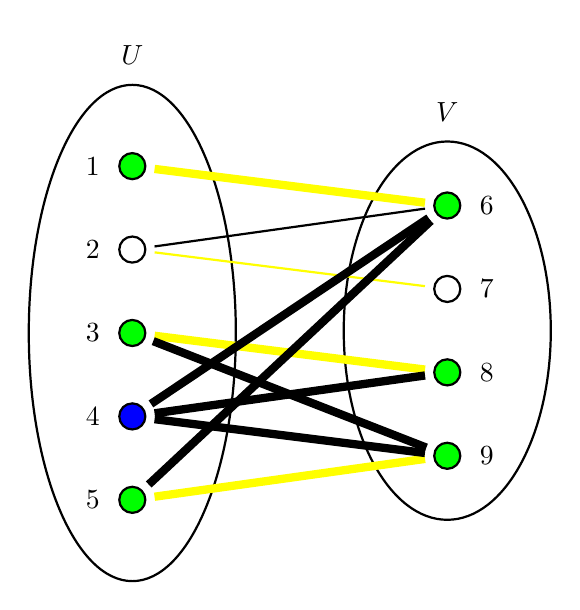
\begin{tikzpicture}[thick,
        every node/.style={draw,circle},
        fsnode/.style={fill=myblue},
        ssnode/.style={fill=mygreen},
        every fit/.style={ellipse,draw,inner sep=-2pt,text width=2cm},
        shorten >= 3pt,shorten <= 3pt
        ]
        
        % the vertices of U
        \begin{scope}[start chain=going below,node distance=7mm]
        \node[fsnode,on chain,fill=mygreen] (f1) [label=left: 1] {};
        \node[fsnode,on chain,fill=white] (f2) [label=left: 2] {};
        \node[fsnode,on chain,fill=mygreen] (f3) [label=left: 3] {};
        \node[fsnode,on chain,fill=myblue] (f4) [label=left: 4] {};
        \node[fsnode,on chain,fill=mygreen] (f5) [label=left: 5] {};
        \end{scope}
        
        % the vertices of V
        \begin{scope}[xshift=4cm,yshift=-0.5cm,start chain=going below,node distance=7mm]
        \node[ssnode,on chain,fill=mygreen] (s6) [label=right: 6] {};
        \node[ssnode,on chain,fill=white] (s7) [label=right: 7] {};
        \node[ssnode,on chain,fill=mygreen] (s8) [label=right: 8] {};
        \node[ssnode,on chain,fill=mygreen] (s9) [label=right: 9] {};
        \end{scope}
        
        % the set U
        \node [black,fit=(f1) (f5),label=above:$U$] {};
        % the set V
        \node [black,fit=(s6) (s9),label=above:$V$] {};
        
        % the edges
        \draw (f1) -- (s6) [color=myred,line width=3pt];
        \draw (s6) -- (f2) [];
        \draw (f2) -- (s7) [color=myred];
        \draw (s8) -- (f3) [color=myred,line width=3pt];
        \draw (f3) -- (s9) [line width=3pt];
        \draw (s9) -- (f5) [color=myred,line width=3pt];
        \draw (f5) -- (s6) [line width=3pt];
        \draw (f4) -- (s6) [line width=3pt];
        \draw (f4) -- (s8) [line width=3pt];
        \draw (f4) -- (s9) [line width=3pt];
        \end{tikzpicture}\only<6>{\hspace{2cm}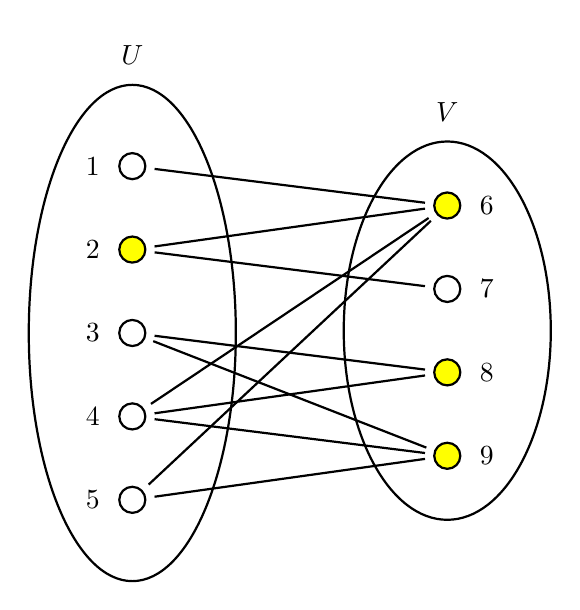
\begin{tikzpicture}[thick,
        every node/.style={draw,circle},
        fsnode/.style={fill=myblue},
        ssnode/.style={fill=mygreen},
        every fit/.style={ellipse,draw,inner sep=-2pt,text width=2cm},
        shorten >= 3pt,shorten <= 3pt
        ]
        
        % the vertices of U
        \begin{scope}[start chain=going below,node distance=7mm]
        \node[fsnode,on chain,fill=white] (f1) [label=left: 1] {};
        \node[fsnode,on chain,fill=mymauve] (f2) [label=left: 2] {};
        \node[fsnode,on chain,fill=white] (f3) [label=left: 3] {};
        \node[fsnode,on chain,fill=white] (f4) [label=left: 4] {};
        \node[fsnode,on chain,fill=white] (f5) [label=left: 5] {};
        \end{scope}
        
        % the vertices of V
        \begin{scope}[xshift=4cm,yshift=-0.5cm,start chain=going below,node distance=7mm]
        \node[ssnode,on chain,fill=mymauve] (s6) [label=right: 6] {};
        \node[ssnode,on chain,fill=white] (s7) [label=right: 7] {};
        \node[ssnode,on chain,fill=mymauve] (s8) [label=right: 8] {};
        \node[ssnode,on chain,fill=mymauve] (s9) [label=right: 9] {};
        \end{scope}
        
        % the set U
        \node [black,fit=(f1) (f5),label=above:$U$] {};
        % the set V
        \node [black,fit=(s6) (s9),label=above:$V$] {};
        
        % the edges
        \draw (f1) -- (s6) [];
        \draw (s6) -- (f2) [];
        \draw (f2) -- (s7) [];
        \draw (s8) -- (f3) [];
        \draw (f3) -- (s9) [];
        \draw (s9) -- (f5) [];
        \draw (f5) -- (s6) [];
        \draw (f4) -- (s6) [];
        \draw (f4) -- (s8) [];
        \draw (f4) -- (s9) [];
        \end{tikzpicture}}}
    
    \only<5-6>{Then $\textcolor{mymauve}K = (U \backslash \textcolor{mygreen}{Z})\cup(V\cap \textcolor{mygreen}{Z})$ is a minimum vertex cover}
\end{frame}
\begin{frame}{Maximum independant set (in bipartite graph)}
    An \textbf{independant set} of a bipartite graph $G=<V,E>$ is a set of nodes $MIS$ such that there is no edges between nodes in $MIS$.\\
    \vspace{1cm}
    
    Said in another way, $\not\exists v_1\in MIS, v_2 \in MIS$ s.t. $(v_1,v_2) \in E$.\\
    \vspace{1cm}
    
    A \textbf{maximum independant set} is an independant set whose size is maximal (...)
\end{frame}
\begin{frame}{Maximum independant set (2)}
    Given a Minimum vertex cover $K$ on a graph with the set of nodes $S=U+V$, then
    $$\textcolor{mygray}{MIS}=S-\textcolor{mymauve}{K}$$
    is a maximum independant set.
    \centering
    \scalebox{0.6}{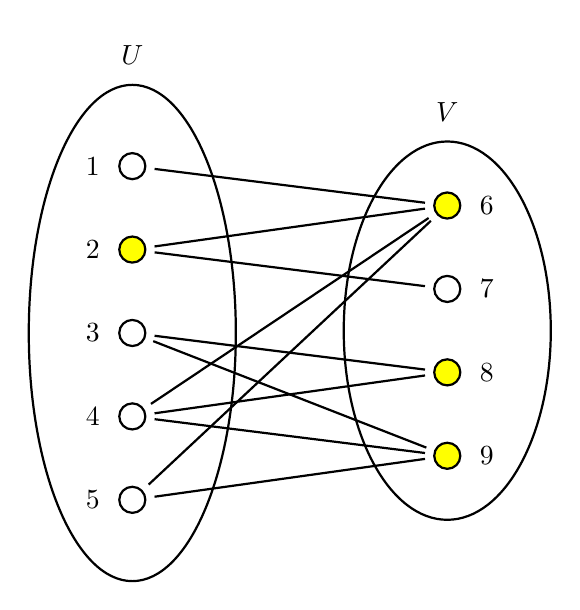
\begin{tikzpicture}[thick,
        every node/.style={draw,circle},
        fsnode/.style={fill=myblue},
        ssnode/.style={fill=mygreen},
        every fit/.style={ellipse,draw,inner sep=-2pt,text width=2cm},
        shorten >= 3pt,shorten <= 3pt
        ]
        
        % the vertices of U
        \begin{scope}[start chain=going below,node distance=7mm]
        \node[fsnode,on chain,fill=white] (f1) [label=left: 1] {};
        \node[fsnode,on chain,fill=mymauve] (f2) [label=left: 2] {};
        \node[fsnode,on chain,fill=white] (f3) [label=left: 3] {};
        \node[fsnode,on chain,fill=white] (f4) [label=left: 4] {};
        \node[fsnode,on chain,fill=white] (f5) [label=left: 5] {};
        \end{scope}
        
        % the vertices of V
        \begin{scope}[xshift=4cm,yshift=-0.5cm,start chain=going below,node distance=7mm]
        \node[ssnode,on chain,fill=mymauve] (s6) [label=right: 6] {};
        \node[ssnode,on chain,fill=white] (s7) [label=right: 7] {};
        \node[ssnode,on chain,fill=mymauve] (s8) [label=right: 8] {};
        \node[ssnode,on chain,fill=mymauve] (s9) [label=right: 9] {};
        \end{scope}
        
        % the set U
        \node [black,fit=(f1) (f5),label=above:$U$] {};
        % the set V
        \node [black,fit=(s6) (s9),label=above:$V$] {};
        
        % the edges
        \draw (f1) -- (s6) [];
        \draw (s6) -- (f2) [];
        \draw (f2) -- (s7) [];
        \draw (s8) -- (f3) [];
        \draw (f3) -- (s9) [];
        \draw (s9) -- (f5) [];
        \draw (f5) -- (s6) [];
        \draw (f4) -- (s6) [];
        \draw (f4) -- (s8) [];
        \draw (f4) -- (s9) [];
        \end{tikzpicture}\hspace{2cm}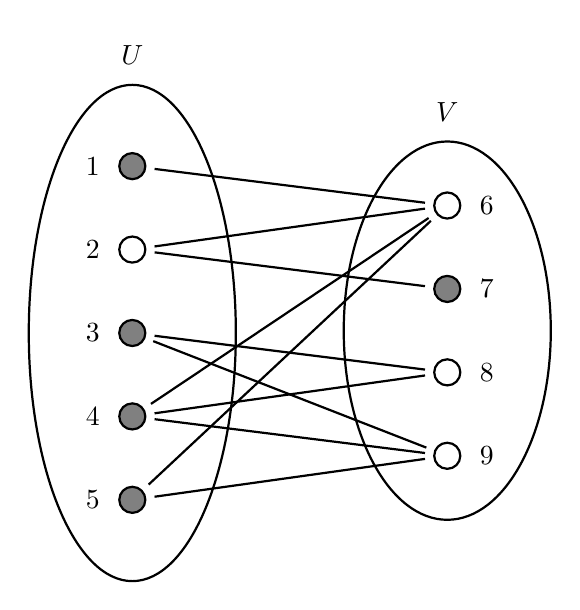
\begin{tikzpicture}[thick,
        every node/.style={draw,circle},
        fsnode/.style={fill=myblue},
        ssnode/.style={fill=mygreen},
        every fit/.style={ellipse,draw,inner sep=-2pt,text width=2cm},
        shorten >= 3pt,shorten <= 3pt
        ]
        
        % the vertices of U
        \begin{scope}[start chain=going below,node distance=7mm]
        \node[fsnode,on chain,fill=mygray] (f1) [label=left: 1] {};
        \node[fsnode,on chain,fill=white] (f2) [label=left: 2] {};
        \node[fsnode,on chain,fill=mygray] (f3) [label=left: 3] {};
        \node[fsnode,on chain,fill=mygray] (f4) [label=left: 4] {};
        \node[fsnode,on chain,fill=mygray] (f5) [label=left: 5] {};
        \end{scope}
        
        % the vertices of V
        \begin{scope}[xshift=4cm,yshift=-0.5cm,start chain=going below,node distance=7mm]
        \node[ssnode,on chain,fill=white] (s6) [label=right: 6] {};
        \node[ssnode,on chain,fill=mygray] (s7) [label=right: 7] {};
        \node[ssnode,on chain,fill=white] (s8) [label=right: 8] {};
        \node[ssnode,on chain,fill=white] (s9) [label=right: 9] {};
        \end{scope}
        
        % the set U
        \node [black,fit=(f1) (f5),label=above:$U$] {};
        % the set V
        \node [black,fit=(s6) (s9),label=above:$V$] {};
        
        % the edges
        \draw (f1) -- (s6) [];
        \draw (s6) -- (f2) [];
        \draw (f2) -- (s7) [];
        \draw (s8) -- (f3) [];
        \draw (f3) -- (s9) [];
        \draw (s9) -- (f5) [];
        \draw (f5) -- (s6) [];
        \draw (f4) -- (s6) [];
        \draw (f4) -- (s8) [];
        \draw (f4) -- (s9) [];
        \end{tikzpicture}}
\end{frame}
\end{document}



